%%%%%%%%%%%%%%%%%%%%%%%%%%%%%%%%%%%%%%%%%%%%%%%%%%%%%%%%%
%COPYRIGHT
%%%%%%%%%%%%%%%%%%%%%%%%%%%%%%%%%%%%%%%%%%%%%%%%%%%%%%%%%


    % Copyright (C) 2016 Manuel Castillo López

    % This program is free software: you can redistribute it and/or modify
    % it under the terms of the GNU General Public License as published by
    % the Free Software Foundation, either version 3 of the License, or
    % (at your option) any later version.

    % This program is distributed in the hope that it will be useful,
    % but WITHOUT ANY WARRANTY; without even the implied warranty of
    % MERCHANTABILITY or FITNESS FOR A PARTICULAR PURPOSE.  See the
    % GNU General Public License for more details.

    % You should have received a copy of the GNU General Public License
    % along with this program.  If not, see <http://www.gnu.org/licenses/>.

\documentclass[0_algebra.tex]{subfiles}
\begin{document}


\onlyinsubfile{
\title{\centering \huge \bfseries Álgebra Lineal}
\author{
	\emph{ \bfseries \centering Tema 1: Conceptos básicos}\\[1.5 cm]
 %	\emph{\centering Open Source Project}\\[1.5 cm]
 % 	\textsc{Escuela Técnica Superior de Ingeniería Industrial}\\
 % 	\textsc{University of Málaga}\\[0.5 cm]
 	\texttt{ingenierocontracabrones.blogspot.com}\\[0.5 cm]
	\texttt{mclnaranjito@gmail.com}\\[4 cm]
	\small{Copyright \copyright \ (2016 - \the\year) \ Manuel Castillo López.} \\
	\small{GPL GNU General Public License}\\[0.5 cm]
	}
\maketitle
\tableofcontents
}

\chapter{Conceptos básicos I}
Para comenzar el estudio del álgebra lineal, es preciso introducir conceptos pertenecientes al álgebra abstracta:
\section{Conjuntos}
Un conjunto es una reunión de determinados objetos bien definidos y diferenciables los unos de los otros. A modo de ejemplo tenemos los siguientes conjuntos numéricos:

\begin{itemize}
\item Los números naturales: $\mathbb{N}=\lbrace 0,1,2,3,... \rbrace$
\item Los números enteros: $\mathbb{Z}=\lbrace ...,-3,-2,-1,0,1,2,3,... \rbrace$
\item Los números racionales: $\mathbb{Q}=\lbrace \frac{a}{b}:\ a,b\in \mathbb{Z},\ b\neq 0 \rbrace$
\item Los números iracionales: $\mathbb{I}=\lbrace \sqrt{2}, \sqrt{5}, \pi, e, \ldots  \rbrace$
\item Los números reales: $\mathbb{R}=\lbrace \mathbb{Q} \cup \mathbb{I}\rbrace$
\item Los números complejos: $\mathbb{C}=\lbrace a+bi: a,b\in \mathbb{R}\rbrace$
\end{itemize}

Sea A un conjunto numérico. Denotaremos por $A^*$ al conjunto de elementos de $A$ salvo el cero, mientras que $A^+$ y $A^-$ designan a los elementos positivos y negativos de $A$ respectivamente. Por ejemplo, $\mathbb{N}^*=\lbrace 1,2,3,... \rbrace = \mathbb{Z}^+$, $\mathbb{Z}^-=\lbrace ...,-3,-2,-1\rbrace$\\

Al número de elementos de A lo denominamos cardinal de A y se denota por $card(A)$


\subsection*{Operaciones entre conjuntos}
Sean $A$ y $B$ como dos conjuntos contenidos en un tercero $E$. Las operaciones básicas que se pueden realizar entre ellos son las siguientes:

\begin{itemize}
    \item Inclusión: $A\subset B \equiv \lbrace x: \ x \in A \Rightarrow x \in B \rbrace$
\begin{figure}[h]
\centering

%%%%%%%%%%%%%%%%%%%%%%%%%%%%%%%%%%%%%%%%%%%%%%%%%%%%%%%%%%
%COPYRIGHT
%%%%%%%%%%%%%%%%%%%%%%%%%%%%%%%%%%%%%%%%%%%%%%%%%%%%%%%%%


    % Copyright (C) 2016 Manuel Castillo López

    % This program is free software: you can redistribute it and/or modify
    % it under the terms of the GNU General Public License as published by
    % the Free Software Foundation, either version 3 of the License, or
    % (at your option) any later version.

    % This program is distributed in the hope that it will be useful,
    % but WITHOUT ANY WARRANTY; without even the implied warranty of
    % MERCHANTABILITY or FITNESS FOR A PARTICULAR PURPOSE.  See the
    % GNU General Public License for more details.

    % You should have received a copy of the GNU General Public License
    % along with this program.  If not, see <http://www.gnu.org/licenses/>.


%%%%%%%%%%%%%%%%%%%%%%%%%%%%%%%%%%%%%%%%%%%%%%%%%%%%%%%%%
%TIPO Y ESTILO DEL DOCUMENTO
%%%%%%%%%%%%%%%%%%%%%%%%%%%%%%%%%%%%%%%%%%%%%%%%%%%%%%%%%

	\documentclass[12pt,a4paper]{book}
	\usepackage[spanish]{babel}%Español
	\usepackage[utf8]{inputenc}%Tildes
	\usepackage{makeidx}%Índice
	\usepackage[toc,page]{appendix}

%Hiperenlaces
	%Para url: \hyperref{htto://www...}{texto}
	\usepackage[colorlinks]{hyperref}
	\usepackage{color}
	\definecolor{darkred}{rgb}{0.5,0,0}
	\definecolor{darkgreen}{rgb}{0,0.5,0}
	\definecolor{darkblue}{rgb}{0,0.2,0.4}
	\hypersetup{
    	colorlinks=true,%
    	citecolor=darkblue,%
    	filecolor=darkgreen,%
    	linkcolor=darkblue,%
    	urlcolor=darkred
	}

%Modificaciones
	%\renewcommand{\appendixname}{Anexo}%Para el apéndice
	%\renewcommand{\appendixtocname}{Anexo}
	%\renewcommand{\appendixpagename}{Anexo}
	%\addto\captionsspanish{\renewcommand{\tablename}{Tabla}} %Para las tablas
	%\addto\captionsspanish{\renewcommand{\chaptername}{Apartado}} %Cambia el nombre del capítulo

%%%%%%%%%%%%%%%%%%%%%%%%%%%%%%%%%%%%%%%%%%%%%%%%%%%%%%%%%
%CONFIGURACIÓN DE PÁGINA
%%%%%%%%%%%%%%%%%%%%%%%%%%%%%%%%%%%%%%%%%%%%%%%%%%%%%%%%%

	%\usepackage[left=2.5cm,right=2.5cm,top=3cm,bottom=3cm]{geometry} %Márgenes
	%\usepackage{setspace} %Permite usar setstretch
	%\setstretch{1.3} %Interlineado
	%\setlength\parindent{0cm} %Sangría
%	\usepackage{fancyhdr} %Para fancy style
%	\pagestyle{fancy}
%		\lhead{}
%		\chead{}
%		\lfoot{}
%		\cfoot{\thepage}	\rfoot{\href{ingenierocontracabrones.blogspot.com}{ingenierocontracabrones}}

\usepackage{fancyhdr}
\setlength{\headheight}{15pt}

\pagestyle{fancy}

\renewcommand{\chaptermark}[1]{ \markboth{#1}{} }
\renewcommand{\sectionmark}[1]{ \markright{#1} }

\fancyhf{}
\fancyhead[LE,RO]{\thepage}
\fancyhead[RE]{\textit{ \nouppercase{\leftmark}} }
\fancyhead[LO]{\textit{ \nouppercase{\rightmark}} }

\fancypagestyle{plain}{ %
  \fancyhf{} % remove everything
  \renewcommand{\headrulewidth}{0pt} % remove lines as well
  \renewcommand{\footrulewidth}{0pt}
}
%\rfoot{\href{ingenierocontracabrones.blogspot.com}{ICC}}

%%%%%%%%%%%%%%%%%%%%%%%%%%%%%%%%%%%%%%%%%%%%%%%%%%%%%%%%%
%GRÁFICAS
%%%%%%%%%%%%%%%%%%%%%%%%%%%%%%%%%%%%%%%%%%%%%%%%%%%%%%%%%

	\usepackage{graphicx}%Gráficas
	\graphicspath{{./imagenes/}}%Fichero donde guardo las gráficas
	\usepackage{epstopdf}%Imágenes postscript+
	\usepackage{tikz}
	\usepackage{tikz-3dplot}
	\usepackage{siunitx}


	%Frame colors
	\definecolor{a_color}{RGB}{0,0,200}%Blue
	\definecolor{e_color}{RGB}{0,100,0}%Green
	\definecolor{f_color}{RGB}{100,50,0}%Orange
	\definecolor{b_color}{RGB}{200,0,0}%Red

%%%%%%%%%%%%%%%%%%%%%%%%%%%%%%%%%%%%%%%%%%%%%%%%%%%%%%%%%
%MATEMÁTICAS
%%%%%%%%%%%%%%%%%%%%%%%%%%%%%%%%%%%%%%%%%%%%%%%%%%%%%%%%%
	\usepackage{mathtools}%Librería matemática
	\usepackage{amssymb}%Símbolos matemáticos
	\usepackage{cancel}%Para usar el cancelto
	\usepackage[]{algorithm2e}

%%%%%%%%%%%%%%%%%%%%%%%%%%%%%%%%%%%%%%%%%%%%%%%%%%%%%%%%%
%	SUBFILES
%%%%%%%%%%%%%%%%%%%%%%%%%%%%%%%%%%%%%%%%%%%%%%%%%%%%%%%%%
	\usepackage{subfiles}
	\newcommand{\onlyinsubfile}[1]{#1}
	\newcommand{\notinsubfile}[1]{}

%%%%%%%%%%%%%%%%%%%%%%%%%%%%%%%%%%%%%%%%%%%%%%%%%%%%%%%%%
% TÍTULO POR DEFECTO
%%%%%%%%%%%%%%%%%%%%%%%%%%%%%%%%%%%%%%%%%%%%%%%%%%%%%%%%%
\title{\centering \huge \bfseries Álgebra Lineal}
\author{
	\emph{\centering Contenido completo}\\[1.5 cm]
 %	\emph{\centering Open Source Project}\\[1.5 cm]
 % 	\textsc{Escuela Técnica Superior de Ingeniería Industrial}\\
 % 	\textsc{University of Málaga}\\[0.5 cm]
 	\texttt{ingenierocontracabrones.blogspot.com}\\[0.5 cm]
	\texttt{mclnaranjito@gmail.com}\\[4 cm]
	\small{Copyright \copyright \ (2016 - \the\year) \ Manuel Castillo López.} \\
	\small{GPL GNU General Public License}\\[0.5 cm]
	}

%\input{../../../paquetes_tikz.tex}

%\begin{document}

% Definition of circles
\def\firstcircle{(0,0) circle (1.5cm)}
\def\secondcircle{(0:2cm) circle (1.5cm)}
\def\square{(-2,-2) [rounded corners]rectangle (4,2)}

\colorlet{circle edge}{black}
\colorlet{circle area}{red!30}

\tikzset{filled/.style={fill=circle area, draw=circle edge, thick},
    outline/.style={draw=circle edge, thick}}

\setlength{\parskip}{5mm}

\begin{tikzpicture}[scale=0.75]
    \draw[outline] (1,0) circle (1.5cm) node [above]{$B$};
    \draw[filled] (0.5,-0.7) circle (0.5cm) node {$A$};                             ;
    \draw[outline] \square node [below left] {$E$};
    \node[anchor=south] at (current bounding box.north) {$A\subset B$};
\end{tikzpicture}
%\end{document}
\end{figure}

\item Unión: $A \cup B \equiv \lbrace x: \ x \in A\ \text{ó} \ x \in B\rbrace$

\begin{figure}[h]
\centering
\input{img/tema1/conjuntos/union.tex}
\end{figure}

\item Intersección: $A \cap B \equiv \lbrace x: \ x \in A\ \text{y} \ x \in B\rbrace$

\begin{figure}[h]
\centering

%%%%%%%%%%%%%%%%%%%%%%%%%%%%%%%%%%%%%%%%%%%%%%%%%%%%%%%%%%
%COPYRIGHT
%%%%%%%%%%%%%%%%%%%%%%%%%%%%%%%%%%%%%%%%%%%%%%%%%%%%%%%%%


    % Copyright (C) 2016 Manuel Castillo López

    % This program is free software: you can redistribute it and/or modify
    % it under the terms of the GNU General Public License as published by
    % the Free Software Foundation, either version 3 of the License, or
    % (at your option) any later version.

    % This program is distributed in the hope that it will be useful,
    % but WITHOUT ANY WARRANTY; without even the implied warranty of
    % MERCHANTABILITY or FITNESS FOR A PARTICULAR PURPOSE.  See the
    % GNU General Public License for more details.

    % You should have received a copy of the GNU General Public License
    % along with this program.  If not, see <http://www.gnu.org/licenses/>.


%%%%%%%%%%%%%%%%%%%%%%%%%%%%%%%%%%%%%%%%%%%%%%%%%%%%%%%%%
%TIPO Y ESTILO DEL DOCUMENTO
%%%%%%%%%%%%%%%%%%%%%%%%%%%%%%%%%%%%%%%%%%%%%%%%%%%%%%%%%

	\documentclass[12pt,a4paper]{book}
	\usepackage[spanish]{babel}%Español
	\usepackage[utf8]{inputenc}%Tildes
	\usepackage{makeidx}%Índice
	\usepackage[toc,page]{appendix}

%Hiperenlaces
	%Para url: \hyperref{htto://www...}{texto}
	\usepackage[colorlinks]{hyperref}
	\usepackage{color}
	\definecolor{darkred}{rgb}{0.5,0,0}
	\definecolor{darkgreen}{rgb}{0,0.5,0}
	\definecolor{darkblue}{rgb}{0,0.2,0.4}
	\hypersetup{
    	colorlinks=true,%
    	citecolor=darkblue,%
    	filecolor=darkgreen,%
    	linkcolor=darkblue,%
    	urlcolor=darkred
	}

%Modificaciones
	%\renewcommand{\appendixname}{Anexo}%Para el apéndice
	%\renewcommand{\appendixtocname}{Anexo}
	%\renewcommand{\appendixpagename}{Anexo}
	%\addto\captionsspanish{\renewcommand{\tablename}{Tabla}} %Para las tablas
	%\addto\captionsspanish{\renewcommand{\chaptername}{Apartado}} %Cambia el nombre del capítulo

%%%%%%%%%%%%%%%%%%%%%%%%%%%%%%%%%%%%%%%%%%%%%%%%%%%%%%%%%
%CONFIGURACIÓN DE PÁGINA
%%%%%%%%%%%%%%%%%%%%%%%%%%%%%%%%%%%%%%%%%%%%%%%%%%%%%%%%%

	%\usepackage[left=2.5cm,right=2.5cm,top=3cm,bottom=3cm]{geometry} %Márgenes
	%\usepackage{setspace} %Permite usar setstretch
	%\setstretch{1.3} %Interlineado
	%\setlength\parindent{0cm} %Sangría
%	\usepackage{fancyhdr} %Para fancy style
%	\pagestyle{fancy}
%		\lhead{}
%		\chead{}
%		\lfoot{}
%		\cfoot{\thepage}	\rfoot{\href{ingenierocontracabrones.blogspot.com}{ingenierocontracabrones}}

\usepackage{fancyhdr}
\setlength{\headheight}{15pt}

\pagestyle{fancy}

\renewcommand{\chaptermark}[1]{ \markboth{#1}{} }
\renewcommand{\sectionmark}[1]{ \markright{#1} }

\fancyhf{}
\fancyhead[LE,RO]{\thepage}
\fancyhead[RE]{\textit{ \nouppercase{\leftmark}} }
\fancyhead[LO]{\textit{ \nouppercase{\rightmark}} }

\fancypagestyle{plain}{ %
  \fancyhf{} % remove everything
  \renewcommand{\headrulewidth}{0pt} % remove lines as well
  \renewcommand{\footrulewidth}{0pt}
}
%\rfoot{\href{ingenierocontracabrones.blogspot.com}{ICC}}

%%%%%%%%%%%%%%%%%%%%%%%%%%%%%%%%%%%%%%%%%%%%%%%%%%%%%%%%%
%GRÁFICAS
%%%%%%%%%%%%%%%%%%%%%%%%%%%%%%%%%%%%%%%%%%%%%%%%%%%%%%%%%

	\usepackage{graphicx}%Gráficas
	\graphicspath{{./imagenes/}}%Fichero donde guardo las gráficas
	\usepackage{epstopdf}%Imágenes postscript+
	\usepackage{tikz}
	\usepackage{tikz-3dplot}
	\usepackage{siunitx}


	%Frame colors
	\definecolor{a_color}{RGB}{0,0,200}%Blue
	\definecolor{e_color}{RGB}{0,100,0}%Green
	\definecolor{f_color}{RGB}{100,50,0}%Orange
	\definecolor{b_color}{RGB}{200,0,0}%Red

%%%%%%%%%%%%%%%%%%%%%%%%%%%%%%%%%%%%%%%%%%%%%%%%%%%%%%%%%
%MATEMÁTICAS
%%%%%%%%%%%%%%%%%%%%%%%%%%%%%%%%%%%%%%%%%%%%%%%%%%%%%%%%%
	\usepackage{mathtools}%Librería matemática
	\usepackage{amssymb}%Símbolos matemáticos
	\usepackage{cancel}%Para usar el cancelto
	\usepackage[]{algorithm2e}

%%%%%%%%%%%%%%%%%%%%%%%%%%%%%%%%%%%%%%%%%%%%%%%%%%%%%%%%%
%	SUBFILES
%%%%%%%%%%%%%%%%%%%%%%%%%%%%%%%%%%%%%%%%%%%%%%%%%%%%%%%%%
	\usepackage{subfiles}
	\newcommand{\onlyinsubfile}[1]{#1}
	\newcommand{\notinsubfile}[1]{}

%%%%%%%%%%%%%%%%%%%%%%%%%%%%%%%%%%%%%%%%%%%%%%%%%%%%%%%%%
% TÍTULO POR DEFECTO
%%%%%%%%%%%%%%%%%%%%%%%%%%%%%%%%%%%%%%%%%%%%%%%%%%%%%%%%%
\title{\centering \huge \bfseries Álgebra Lineal}
\author{
	\emph{\centering Contenido completo}\\[1.5 cm]
 %	\emph{\centering Open Source Project}\\[1.5 cm]
 % 	\textsc{Escuela Técnica Superior de Ingeniería Industrial}\\
 % 	\textsc{University of Málaga}\\[0.5 cm]
 	\texttt{ingenierocontracabrones.blogspot.com}\\[0.5 cm]
	\texttt{mclnaranjito@gmail.com}\\[4 cm]
	\small{Copyright \copyright \ (2016 - \the\year) \ Manuel Castillo López.} \\
	\small{GPL GNU General Public License}\\[0.5 cm]
	}

%\input{../../../paquetes_tikz.tex}

%\begin{document}

% Definition of circles
\def\firstcircle{(0,0) circle (1.5cm)}
\def\secondcircle{(0:2cm) circle (1.5cm)}
\def\square{(-2,-2) [rounded corners]rectangle (4,2)}

\colorlet{circle edge}{black}
\colorlet{circle area}{red!30}

\tikzset{filled/.style={fill=circle area, draw=circle edge, thick},
    outline/.style={draw=circle edge, thick}}

\setlength{\parskip}{5mm}


% Set A and B
\begin{tikzpicture}[scale=0.75]
    \begin{scope}
        \clip \firstcircle;
        \fill[filled] \secondcircle;
        \square;
    \end{scope}
    \draw[outline] \firstcircle node {$A$};
    \draw[outline] \secondcircle node {$B$};
    \draw[outline] \square node [below left] {$E$};
    \node[anchor=south] at (current bounding box.north) {$A \cap B$};
\end{tikzpicture}


%\end{document}
\end{figure}
\newpage

\item Contrario o complementario: $A^c = \overline{A} \equiv \lbrace x:\ x \not \in A \rbrace$

\begin{figure}[h]
\centering

%%%%%%%%%%%%%%%%%%%%%%%%%%%%%%%%%%%%%%%%%%%%%%%%%%%%%%%%%%
%COPYRIGHT
%%%%%%%%%%%%%%%%%%%%%%%%%%%%%%%%%%%%%%%%%%%%%%%%%%%%%%%%%


    % Copyright (C) 2016 Manuel Castillo López

    % This program is free software: you can redistribute it and/or modify
    % it under the terms of the GNU General Public License as published by
    % the Free Software Foundation, either version 3 of the License, or
    % (at your option) any later version.

    % This program is distributed in the hope that it will be useful,
    % but WITHOUT ANY WARRANTY; without even the implied warranty of
    % MERCHANTABILITY or FITNESS FOR A PARTICULAR PURPOSE.  See the
    % GNU General Public License for more details.

    % You should have received a copy of the GNU General Public License
    % along with this program.  If not, see <http://www.gnu.org/licenses/>.


%%%%%%%%%%%%%%%%%%%%%%%%%%%%%%%%%%%%%%%%%%%%%%%%%%%%%%%%%
%TIPO Y ESTILO DEL DOCUMENTO
%%%%%%%%%%%%%%%%%%%%%%%%%%%%%%%%%%%%%%%%%%%%%%%%%%%%%%%%%

	\documentclass[12pt,a4paper]{book}
	\usepackage[spanish]{babel}%Español
	\usepackage[utf8]{inputenc}%Tildes
	\usepackage{makeidx}%Índice
	\usepackage[toc,page]{appendix}

%Hiperenlaces
	%Para url: \hyperref{htto://www...}{texto}
	\usepackage[colorlinks]{hyperref}
	\usepackage{color}
	\definecolor{darkred}{rgb}{0.5,0,0}
	\definecolor{darkgreen}{rgb}{0,0.5,0}
	\definecolor{darkblue}{rgb}{0,0.2,0.4}
	\hypersetup{
    	colorlinks=true,%
    	citecolor=darkblue,%
    	filecolor=darkgreen,%
    	linkcolor=darkblue,%
    	urlcolor=darkred
	}

%Modificaciones
	%\renewcommand{\appendixname}{Anexo}%Para el apéndice
	%\renewcommand{\appendixtocname}{Anexo}
	%\renewcommand{\appendixpagename}{Anexo}
	%\addto\captionsspanish{\renewcommand{\tablename}{Tabla}} %Para las tablas
	%\addto\captionsspanish{\renewcommand{\chaptername}{Apartado}} %Cambia el nombre del capítulo

%%%%%%%%%%%%%%%%%%%%%%%%%%%%%%%%%%%%%%%%%%%%%%%%%%%%%%%%%
%CONFIGURACIÓN DE PÁGINA
%%%%%%%%%%%%%%%%%%%%%%%%%%%%%%%%%%%%%%%%%%%%%%%%%%%%%%%%%

	%\usepackage[left=2.5cm,right=2.5cm,top=3cm,bottom=3cm]{geometry} %Márgenes
	%\usepackage{setspace} %Permite usar setstretch
	%\setstretch{1.3} %Interlineado
	%\setlength\parindent{0cm} %Sangría
%	\usepackage{fancyhdr} %Para fancy style
%	\pagestyle{fancy}
%		\lhead{}
%		\chead{}
%		\lfoot{}
%		\cfoot{\thepage}	\rfoot{\href{ingenierocontracabrones.blogspot.com}{ingenierocontracabrones}}

\usepackage{fancyhdr}
\setlength{\headheight}{15pt}

\pagestyle{fancy}

\renewcommand{\chaptermark}[1]{ \markboth{#1}{} }
\renewcommand{\sectionmark}[1]{ \markright{#1} }

\fancyhf{}
\fancyhead[LE,RO]{\thepage}
\fancyhead[RE]{\textit{ \nouppercase{\leftmark}} }
\fancyhead[LO]{\textit{ \nouppercase{\rightmark}} }

\fancypagestyle{plain}{ %
  \fancyhf{} % remove everything
  \renewcommand{\headrulewidth}{0pt} % remove lines as well
  \renewcommand{\footrulewidth}{0pt}
}
%\rfoot{\href{ingenierocontracabrones.blogspot.com}{ICC}}

%%%%%%%%%%%%%%%%%%%%%%%%%%%%%%%%%%%%%%%%%%%%%%%%%%%%%%%%%
%GRÁFICAS
%%%%%%%%%%%%%%%%%%%%%%%%%%%%%%%%%%%%%%%%%%%%%%%%%%%%%%%%%

	\usepackage{graphicx}%Gráficas
	\graphicspath{{./imagenes/}}%Fichero donde guardo las gráficas
	\usepackage{epstopdf}%Imágenes postscript+
	\usepackage{tikz}
	\usepackage{tikz-3dplot}
	\usepackage{siunitx}


	%Frame colors
	\definecolor{a_color}{RGB}{0,0,200}%Blue
	\definecolor{e_color}{RGB}{0,100,0}%Green
	\definecolor{f_color}{RGB}{100,50,0}%Orange
	\definecolor{b_color}{RGB}{200,0,0}%Red

%%%%%%%%%%%%%%%%%%%%%%%%%%%%%%%%%%%%%%%%%%%%%%%%%%%%%%%%%
%MATEMÁTICAS
%%%%%%%%%%%%%%%%%%%%%%%%%%%%%%%%%%%%%%%%%%%%%%%%%%%%%%%%%
	\usepackage{mathtools}%Librería matemática
	\usepackage{amssymb}%Símbolos matemáticos
	\usepackage{cancel}%Para usar el cancelto
	\usepackage[]{algorithm2e}

%%%%%%%%%%%%%%%%%%%%%%%%%%%%%%%%%%%%%%%%%%%%%%%%%%%%%%%%%
%	SUBFILES
%%%%%%%%%%%%%%%%%%%%%%%%%%%%%%%%%%%%%%%%%%%%%%%%%%%%%%%%%
	\usepackage{subfiles}
	\newcommand{\onlyinsubfile}[1]{#1}
	\newcommand{\notinsubfile}[1]{}

%%%%%%%%%%%%%%%%%%%%%%%%%%%%%%%%%%%%%%%%%%%%%%%%%%%%%%%%%
% TÍTULO POR DEFECTO
%%%%%%%%%%%%%%%%%%%%%%%%%%%%%%%%%%%%%%%%%%%%%%%%%%%%%%%%%
\title{\centering \huge \bfseries Álgebra Lineal}
\author{
	\emph{\centering Contenido completo}\\[1.5 cm]
 %	\emph{\centering Open Source Project}\\[1.5 cm]
 % 	\textsc{Escuela Técnica Superior de Ingeniería Industrial}\\
 % 	\textsc{University of Málaga}\\[0.5 cm]
 	\texttt{ingenierocontracabrones.blogspot.com}\\[0.5 cm]
	\texttt{mclnaranjito@gmail.com}\\[4 cm]
	\small{Copyright \copyright \ (2016 - \the\year) \ Manuel Castillo López.} \\
	\small{GPL GNU General Public License}\\[0.5 cm]
	}

%\input{../../../paquetes_tikz.tex}

%\begin{document}

% Definition of circles
\def\firstcircle{(0,0) circle (1.5cm)}
\def\secondcircle{(0:2cm) circle (1.5cm)}
\def\square{(-2,-2) [rounded corners]rectangle (4,2)}

\colorlet{circle edge}{black}
\colorlet{circle area}{red!30}

\tikzset{filled/.style={fill=circle area, draw=circle edge, thick},
    outline/.style={draw=circle edge, thick}}

\setlength{\parskip}{5mm}

%A negado
\begin{tikzpicture}[scale=0.75]
    \draw[filled, even odd rule] \firstcircle node {$A$}
                             \square node [below left] {$E$};
    \draw[outline] \secondcircle node{$B$};
    \node[anchor=south] at (current bounding box.north) {$A^c$};
\end{tikzpicture}

%\end{document}
\end{figure}


\item Diferencia: $A-B= A\backslash B=A\cap B^c=A-(A\cap B)\equiv \lbrace x \in A:\ x \not \in B \rbrace$

\begin{figure}[h]
\centering
\input{img/tema1/conjuntos/diferencia.tex}
\end{figure}

\item Diferencia simétrica: $A\vartriangle B=(A-B)\cup (B-A)$

\begin{figure}[h]
\centering
\input{img/tema1/conjuntos/diferenciasim.tex}
\end{figure}

\end{itemize}

Para operar con $n$ conjuntos emplearemos las siguientes notaciones:
$$
\bigcup_{i=1}^n A_i = A_1 \cup A_2 \cup ... \cup A_n \quad \forall i \not = j
$$

$$
\bigcap_{i=1}^n A_i = A_1 \cap A_2 \cap ... \cap A_n
$$

\subsubsection*{Ejemplo:}
Sea $E=\lbrace 1,2,3,4,5,6,7,8,9,10\rbrace$, $A=\lbrace1,3,6,7,9\rbrace$ y $B=\lbrace2,3,5,7,10\rbrace$. Entonces:
\begin{itemize}
\item $A \cup B =\lbrace 1,2,3,5,6,7,9,10 \rbrace$
\item $A \cap B =\lbrace 3,7 \rbrace$
\item $A^c=\lbrace 2,4,5,8,10 \rbrace$,\quad $B^c= \lbrace 1,4,6,8,9\rbrace$
\item $A-B=\lbrace 1,6,9 \rbrace$, \quad $B-A=\lbrace 2,5,10 \rbrace$
\item $A\vartriangle B= \lbrace 1,2,5,6,9,10 \rbrace$

\end{itemize}

\subsection*{Partición de un conjunto}
Particionar un conjunto E consiste en dividirlo en subconjuntos tales que:
\begin{enumerate}
\item $$A_i \cap A_j =\emptyset$$
\item $$E=\bigcup_{i=1}^n A_i$$
\end{enumerate}

\subsubsection*{Ejemplo:}
Sea $E=\lbrace 1,2,3,4,5,6,7,8,9,10\rbrace$ podemos particionarlo, por ejemplo, en tres subconjuntos de diferentes tamaños: $A=\lbrace 1,2 \rbrace$, $B=\lbrace 3,5,7 \rbrace$ y $C=\lbrace 4,6,8,9,10 \rbrace$. De ésta manera se cumple que:
\begin{itemize}
\item  $A \cap B =\emptyset$, $A \cap C =\emptyset$ y $B \cap C =\emptyset$
\item  $E= A \cup B \cup C$
\end{itemize}

También podemos comprobar que el cardinal de un conjunto es la suma del cardinal de sus particiones:  $card(E)=card(A)+card(B)+card(C)=2+3+5=10$.

\subsection*{Producto cartesiano}
Sean dos conjuntos $A$ y $B$. Se define el producto cartesiano $A\times B$ al conjunto de todos los pares ordenados $(a,b)$ en los que el primer componente pertenece a $A$ y el segundo a $B$, es decir:
$$
A\times B=\lbrace (a,b): a\in A, b\in B \rbrace
$$

\subsubsection*{Ejemplo:}
Sean dos conjuntos $A=\lbrace a,b,c \rbrace$ y $B=\lbrace 1,2,3,4 \rbrace$. Entonces:
$$
A\times B =
\left\lbrace
\begin{matrix}
(a,1) & (a,2) & (a,3) & (a,4)\\
(b,1) & (b,2) & (b,3) & (b,4)\\
(c,1) & (c,2) & (c,3) & (c,4)\\
\end{matrix}
\right\rbrace
$$

\subsection*{Propiedades de los conjuntos}
Para facilitar la comprensión de algunas de las siguientes propiedades podemos utilizar las semejanzas entre las propiedades de las operaciones de conjuntos y las operaciones numéricas. Así, la unión se asemeja a la suma numérica, la intersección al producto, el conjunto vacío sería el equivalente del cero y el complementario equivaldría a un cambio de signo.\\

Sean dos subconjuntos $A$, $B$ y $C$ pertenecientes al conjunto $E$. Se dice que las partes de E $P(E)$ forman un Álgebra de Boole si se cumplen las siguientes propiedades.\\

\begin{enumerate}
\item Idempotente:\quad $A\cap A=A$\quad  $A\cup A=A$
\item De complemento:\quad $A\cap A^c=\emptyset$\quad  $A\cup A^c=E$
\item Conmutativa:\quad $A\cap B=B\cap A$\quad  $A\cup B=B\cup A$
\item Asociativa:\quad $(A\cup B)\cup C=A\cup (B\cup C)$

\hspace{3.14 cm}  $(A\cap B)\cap C=A\cap (B\cap C)$
\item Distributiva:\ \ $A\cap (B\cup C)=(A\cap B)\cup (A\cap C)$

\hspace{2.4 cm} $A\cup (B\cap C)=(A\cup B)\cap (A\cup C)$
\item Elemento absorbente:\quad $A\cap \emptyset=\emptyset$\quad  $A\cup E=E$
\item Elemento neutro:\quad $A\cup \emptyset=A$\quad  $A\cap E=A$
\item Simplificativa:\quad $A\cap(A\cup B)=A$\quad  $A\cup(A\cap B)=A$
\item Leyes de Morgan:\quad  $(A\cup B)^c=A^c \cap B^c$ \quad  $(A\cap B)^c=A^c\cup B^c$\\
\end{enumerate}

El lector puede comprobar el cumplimiento de todas estas propiedades gráficamente o numéricamente definiendo los conjuntos A, B, C y E.
\newpage
\section{Relaciones binarias}

Se denomina relación binaria a la vinculación de dos elementos (a y b por ejemplo) y se denota por $aRb$.\\

Sean dos conjuntos $A$ y $B$. Se llama grafo a cualquier subconjunto $G$ del producto cartesiano $A\times B$.
$$
G \subset A\times B
$$

Se dirá que $a\in A$ está relacionado con $b\in B$ a través de $G$ $(aR_Gb)$ si el par ordenado $(a,b)$ pertenece a G.

$$
aR_Gb \Leftrightarrow (a,b) \in G
$$

\subsubsection*{Ejemplo:}

Tomemos el mismo ejemplo que usamos para el producto cartesiano. Sean dos conjuntos $A=\lbrace a,b,c \rbrace$ y $B=\lbrace 1,2,3,4 \rbrace$. Definiremos el grafo

$$
G=\lbrace (a,1),(b,2),(b,3),(c,3),(c,4) \rbrace
$$

De ésta manera, tenemos en $G$ qué elementos de $A$ que están relacionados con qué elementos de $B$ mediante pares ordenados $(a,b)$. Así tenemos, por ejemplo, que $bR_G2$ y que $cR_G3$.\\

Otra forma de establecer una relación es mediante una propiedad $p$. Así diremos que

$$
aRb \Leftrightarrow p(a,b) \text{ es cierta}
$$

\subsubsection*{Ejemplo:}

Sean los conjuntos $A=\lbrace 1,3,5,7 \rbrace$ y $B=\lbrace 2,4,6,8 \rbrace$ y tomemos como propiedad $p(a,b)=a>b$. De ésta manera podemos construir el grafo donde quedan incluidas todas las relaciones que cumplen dicha propiedad:

$$
aRb \Leftrightarrow a>b \Rightarrow G=\lbrace(3,2),(5,2),(5,4),(7,2),(7,4),(7,6) \rbrace
$$

\newpage
\subsubsection*{Propiedades de las relaciones binarias}
\begin{itemize}
\item Reflexiva: $aRa,\ \forall a \in A$
\item Simétrica: $aRb \Rightarrow bRa$
\item Antisimétrica: $aRb\ y\ bRa \Rightarrow a=b$
\item Transitiva: $aRb\ y\ bRc \Rightarrow aRc$
\item Antirreflexiva: $a\cancel{R} a,\ \forall a \in A$
\item Conexa: $aRb$ ó $bRa$, $\forall (a,b) \in A\times A$, $a\not = b$
\item Euclídea: $aRb$ y $aRc$ $\Rightarrow bRc$
\end{itemize}

\subsection*{Relaciones binarias de equivalencia}
Se dice que una relación binaria es de equivalencia si verifica las propiedades reflexiva, simétrica y transitiva. Se denota por $a \sim b$.
$$
R \text{ es de equivalencia } \Leftrightarrow \ R \text{ es }
\begin{cases}
\text{Reflexiva}\\
\text{Simétrica}\\
\text{Transitiva}
\end{cases}
$$

\subsubsection*{Clase de equivalencia}
Sea $A$ un conjunto y $\sim$ una relación binaria de equivalencia definida en $A$. Se denomina clase de equivalencia del elemento $a\in A$, denotada por $[a]$ o por $\overline{a}$, al subconjunto de $A$ formado por todos los elementos relacionados con $a$, es decir,

$$
[a]\equiv \lbrace b \in A : a \sim b \rbrace
$$

Puesto que las relaciones de equivalencia, por definición, son transitivas y simétricas podemos afirmar que la clase de equivalencia de dos elementos relacionados es la misma y, por tanto, cualquiera de los elementos puede representar a dicha clase.

\begin{equation}
a\sim b \Leftrightarrow [a]=[b]
\label{eq1}
\end{equation}



Además podemos afirmar que dos elementos no relacionados pertenecen a distintas clases de equivalencia.

\begin{equation}
a \not \sim b \Leftrightarrow [a] \cap [b] = \emptyset
\label{eq2}
\end{equation}

Basándonos en lo deducido en las expresiones \ref{eq1} y \ref{eq2}, podemos afirmar que cada clase de equivalencia define una partición del conjunto $A$ ya que se cumplen las expresiones \ref{eq3} y \ref{eq4}.

\begin{equation}
A=\bigcup_{i=1}^n [a_i]
\label{eq3}
\end{equation}


\begin{equation}
[a_i]\cap [a_j]=\emptyset \quad \text{si\quad }a_i \not\sim a_j
\label{eq4}
\end{equation}

\subsubsection*{Conjunto cociente}
Al conjunto de todas las clases de equivalencia del conjunto $A$ se le llama conjunto cociente, y se representa por $A/\sim$.

$$
A/\sim \equiv \lbrace [a_i] : a_i \in A \rbrace
$$

\subsubsection*{Ejemplo:}
Sea $A=\lbrace 1,2,3,4,5\rbrace$ y el grafo
$$
G=\lbrace (1,1), (2,2), (3,3), (4,4), (5,5), (1,3), (3,1), (2,4), (4,2) \rbrace
$$

Apoyándonos en la Figura \ref{sagital}, comprobamos que es relación binaria de equivalencia ya que es reflexiva, simétrica y transitiva.\\

\begin{figure}[h]
\centering
%%%%%%%%%%%%%%%%%%%%%%%%%%%%%%%%%%%%%%%%%%%%%%%%%%%%%%%%%%
%COPYRIGHT
%%%%%%%%%%%%%%%%%%%%%%%%%%%%%%%%%%%%%%%%%%%%%%%%%%%%%%%%%


    % Copyright (C) 2016 Manuel Castillo López

    % This program is free software: you can redistribute it and/or modify
    % it under the terms of the GNU General Public License as published by
    % the Free Software Foundation, either version 3 of the License, or
    % (at your option) any later version.

    % This program is distributed in the hope that it will be useful,
    % but WITHOUT ANY WARRANTY; without even the implied warranty of
    % MERCHANTABILITY or FITNESS FOR A PARTICULAR PURPOSE.  See the
    % GNU General Public License for more details.

    % You should have received a copy of the GNU General Public License
    % along with this program.  If not, see <http://www.gnu.org/licenses/>.


%%%%%%%%%%%%%%%%%%%%%%%%%%%%%%%%%%%%%%%%%%%%%%%%%%%%%%%%%
%TIPO Y ESTILO DEL DOCUMENTO
%%%%%%%%%%%%%%%%%%%%%%%%%%%%%%%%%%%%%%%%%%%%%%%%%%%%%%%%%

	\documentclass[12pt,a4paper]{book}
	\usepackage[spanish]{babel}%Español
	\usepackage[utf8]{inputenc}%Tildes
	\usepackage{makeidx}%Índice
	\usepackage[toc,page]{appendix}

%Hiperenlaces
	%Para url: \hyperref{htto://www...}{texto}
	\usepackage[colorlinks]{hyperref}
	\usepackage{color}
	\definecolor{darkred}{rgb}{0.5,0,0}
	\definecolor{darkgreen}{rgb}{0,0.5,0}
	\definecolor{darkblue}{rgb}{0,0.2,0.4}
	\hypersetup{
    	colorlinks=true,%
    	citecolor=darkblue,%
    	filecolor=darkgreen,%
    	linkcolor=darkblue,%
    	urlcolor=darkred
	}

%Modificaciones
	%\renewcommand{\appendixname}{Anexo}%Para el apéndice
	%\renewcommand{\appendixtocname}{Anexo}
	%\renewcommand{\appendixpagename}{Anexo}
	%\addto\captionsspanish{\renewcommand{\tablename}{Tabla}} %Para las tablas
	%\addto\captionsspanish{\renewcommand{\chaptername}{Apartado}} %Cambia el nombre del capítulo

%%%%%%%%%%%%%%%%%%%%%%%%%%%%%%%%%%%%%%%%%%%%%%%%%%%%%%%%%
%CONFIGURACIÓN DE PÁGINA
%%%%%%%%%%%%%%%%%%%%%%%%%%%%%%%%%%%%%%%%%%%%%%%%%%%%%%%%%

	%\usepackage[left=2.5cm,right=2.5cm,top=3cm,bottom=3cm]{geometry} %Márgenes
	%\usepackage{setspace} %Permite usar setstretch
	%\setstretch{1.3} %Interlineado
	%\setlength\parindent{0cm} %Sangría
%	\usepackage{fancyhdr} %Para fancy style
%	\pagestyle{fancy}
%		\lhead{}
%		\chead{}
%		\lfoot{}
%		\cfoot{\thepage}	\rfoot{\href{ingenierocontracabrones.blogspot.com}{ingenierocontracabrones}}

\usepackage{fancyhdr}
\setlength{\headheight}{15pt}

\pagestyle{fancy}

\renewcommand{\chaptermark}[1]{ \markboth{#1}{} }
\renewcommand{\sectionmark}[1]{ \markright{#1} }

\fancyhf{}
\fancyhead[LE,RO]{\thepage}
\fancyhead[RE]{\textit{ \nouppercase{\leftmark}} }
\fancyhead[LO]{\textit{ \nouppercase{\rightmark}} }

\fancypagestyle{plain}{ %
  \fancyhf{} % remove everything
  \renewcommand{\headrulewidth}{0pt} % remove lines as well
  \renewcommand{\footrulewidth}{0pt}
}
%\rfoot{\href{ingenierocontracabrones.blogspot.com}{ICC}}

%%%%%%%%%%%%%%%%%%%%%%%%%%%%%%%%%%%%%%%%%%%%%%%%%%%%%%%%%
%GRÁFICAS
%%%%%%%%%%%%%%%%%%%%%%%%%%%%%%%%%%%%%%%%%%%%%%%%%%%%%%%%%

	\usepackage{graphicx}%Gráficas
	\graphicspath{{./imagenes/}}%Fichero donde guardo las gráficas
	\usepackage{epstopdf}%Imágenes postscript+
	\usepackage{tikz}
	\usepackage{tikz-3dplot}
	\usepackage{siunitx}


	%Frame colors
	\definecolor{a_color}{RGB}{0,0,200}%Blue
	\definecolor{e_color}{RGB}{0,100,0}%Green
	\definecolor{f_color}{RGB}{100,50,0}%Orange
	\definecolor{b_color}{RGB}{200,0,0}%Red

%%%%%%%%%%%%%%%%%%%%%%%%%%%%%%%%%%%%%%%%%%%%%%%%%%%%%%%%%
%MATEMÁTICAS
%%%%%%%%%%%%%%%%%%%%%%%%%%%%%%%%%%%%%%%%%%%%%%%%%%%%%%%%%
	\usepackage{mathtools}%Librería matemática
	\usepackage{amssymb}%Símbolos matemáticos
	\usepackage{cancel}%Para usar el cancelto
	\usepackage[]{algorithm2e}

%%%%%%%%%%%%%%%%%%%%%%%%%%%%%%%%%%%%%%%%%%%%%%%%%%%%%%%%%
%	SUBFILES
%%%%%%%%%%%%%%%%%%%%%%%%%%%%%%%%%%%%%%%%%%%%%%%%%%%%%%%%%
	\usepackage{subfiles}
	\newcommand{\onlyinsubfile}[1]{#1}
	\newcommand{\notinsubfile}[1]{}

%%%%%%%%%%%%%%%%%%%%%%%%%%%%%%%%%%%%%%%%%%%%%%%%%%%%%%%%%
% TÍTULO POR DEFECTO
%%%%%%%%%%%%%%%%%%%%%%%%%%%%%%%%%%%%%%%%%%%%%%%%%%%%%%%%%
\title{\centering \huge \bfseries Álgebra Lineal}
\author{
	\emph{\centering Contenido completo}\\[1.5 cm]
 %	\emph{\centering Open Source Project}\\[1.5 cm]
 % 	\textsc{Escuela Técnica Superior de Ingeniería Industrial}\\
 % 	\textsc{University of Málaga}\\[0.5 cm]
 	\texttt{ingenierocontracabrones.blogspot.com}\\[0.5 cm]
	\texttt{mclnaranjito@gmail.com}\\[4 cm]
	\small{Copyright \copyright \ (2016 - \the\year) \ Manuel Castillo López.} \\
	\small{GPL GNU General Public License}\\[0.5 cm]
	}

%\input{../../../paquetes_tikz.tex}

%\begin{document}
%\tikzstyle{arrow} = [thick,->,>=stealth]

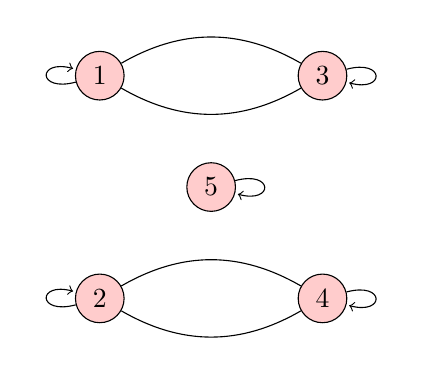
\begin{tikzpicture}[arrow/.style={thick,->,>=stealth},auto,node distance=2cm,main node/.style={circle,fill=red!20,draw}]
  \usetikzlibrary{shapes,arrows}
  
  \node[main node] (1) {1};
  \node[main node] (5) [below right of=1] {5};
  \node[main node] (3) [above right of=5] {3};
  \node[main node] (2) [below left of=5] {2};
  \node[main node] (4) [below right of=5] {4};
  
  \path[]
    (1) edge [loop left]  node {} (1)
    	edge [bend right] node {} (3)
        
    (2) edge [loop left]  node {} (2)
    	edge [bend right] node {} (4)
        
    (3) edge [loop right] node {} (3)
    	edge [bend right] node {} (1)
    	
    (4) edge [loop right] node {} (4)
        edge [bend right] node {} (2)
    
    (5) edge [loop right] node {} (5);
\end{tikzpicture}
%\end{document}
\caption{Diagrama sagital de las relaciones binarias}
\label{sagital}
\end{figure}


Las clases de equivalencia son:

\begin{flalign*}
&[1]= \lbrace 1,3 \rbrace = [3]\\
&[2]= \lbrace 2,4 \rbrace = [4]\\
&[5]= \lbrace 5 \rbrace
\end{flalign*}

Por tanto, el conjunto cociente será:

$$
A/\sim = \lbrace [1],[2],[5] \rbrace
$$
\subsection*{Relaciones binarias de orden}
Se dice que una relación binaria es de orden si verifica las propiedades reflexiva, antisimétrica y transitiva. Se denota por $a \leq b$. Si $a \leq b$ se dice que $a$ es anterior a $b$ o que $b$ es posterior a $a$.
$$
R \text{ es de equivalencia } \Leftrightarrow \ R \text{ es }
\begin{cases}
\text{Reflexiva}\\
\text{Antisimétrica}\\
\text{Transitiva}
\end{cases}
$$

Una relación es de \textbf{orden total} si además es conexa, es decir, todos los elementos están relacionados. Si no es conexa será relación de \textbf{orden parcial}. Se dirá entonces que A está totalmente o parcialmente ordenado si en él hay definida una relación de orden total o parcial respectivamente. Se llama cadena a un subconjunto no vacío totalmente ordenado.\\

Sean $(A,\leq )$ un conjunto ordenado y $B$ un subconjunto no vacío de $A$.\\

Llamamos \textbf{cota superior} de $B$ a cualquier elemento de $A$ que es posterior a todo elemento de $B$. Si existe alguna cota superior, se dice que $B$ está acotado superiormente.\\

Llamamos \textbf{cota inferior} de $B$ a cualquier  elemento de $A$ que es anterior a todo elemento de $B$. Si existe alguna cota inferior, se dice que $B$ está acotado inferiormente.\\

Si $B$ está acotado inferiormente y superiormente, se dirá simplemente que está acotado.\\

\textbf{Extremo superior} de $B$ o \textbf{supremo} de $B$ es la menor de las cotas superiores de $B$. Se denota por $sup_A(B)$. Si el supremo pertenece a $B$, se llama \textbf{máximo.}\\

\textbf{Extremo inferior} de $B$ o \textbf{ínfimo} de $B$ es la mayor de las cotas inferiores de $B$. Se denota por $inf_A(B)$. Si el ínfimo pertenece a $B$, se llama \textbf{mínimo.}\\

Un conjunto se dice que está \textbf{bien ordenado} si todo subconjunto suyo no vacío tiene mínimo.\\

\textbf{Elemento maximal} de $B$ es cualquier elemento de $B$ tal que no existe un elemento posterior a él.\\

\textbf{Elemento minimal} de $B$ es cualquier elemento de $B$ tal que no existe un elemento anterior a él.\\

Un conjunto $A$ ordenado se llamará \textbf{retículo} si todo subconjunto suyo formado por dos elementos posee ínfimo y supremo.\\

\subsubsection*{Ejemplo:}
Sea $A=\lbrace 2,3,5,6,8,16,18 \rbrace$ y consideremos en A la relación de divisibilidad.

$$
\forall x,y \in A \quad x R y \Leftrightarrow x|y
$$

\emph{Inciso: }El término $x|y$ significa $x$ divide a $y$. Ésto se cumple cuando el resto de la división $y/x$ es cero y, por tanto, $y$ es un múltiplo de $x$. En notación matemática sería:

$$
\forall x,y \in \mathbb{Z}\quad x|y \Leftrightarrow \exists \  k \in \mathbb{Z}: y=kx
$$

Puede comprobarse fácilmente que ésta relación es reflexiva, antisimétrica y transitiva. Además, no todos los elementos están relacionados por lo que es de orden parcial.\\

Una herramienta gráfica empleada para las relaciones de orden es el diagrama de Hasse. Está estructurado de abajo a arriba en niveles en función de la anterioridad o posterioridad de cada elemento.\\

Podemos observar, en la figura \ref{hasse}, el diagrama de Hasse de nuestro ejemplo. Comprobamos que los elementos $2$ y $3$ son minimales y los elementos $16$ y $18$ son maximales. El $5$ es minimal y maximal a la vez.\\


\begin{figure}[h]
\centering
%%%%%%%%%%%%%%%%%%%%%%%%%%%%%%%%%%%%%%%%%%%%%%%%%%%%%%%%%%
%COPYRIGHT
%%%%%%%%%%%%%%%%%%%%%%%%%%%%%%%%%%%%%%%%%%%%%%%%%%%%%%%%%


    % Copyright (C) 2016 Manuel Castillo López

    % This program is free software: you can redistribute it and/or modify
    % it under the terms of the GNU General Public License as published by
    % the Free Software Foundation, either version 3 of the License, or
    % (at your option) any later version.

    % This program is distributed in the hope that it will be useful,
    % but WITHOUT ANY WARRANTY; without even the implied warranty of
    % MERCHANTABILITY or FITNESS FOR A PARTICULAR PURPOSE.  See the
    % GNU General Public License for more details.

    % You should have received a copy of the GNU General Public License
    % along with this program.  If not, see <http://www.gnu.org/licenses/>.


%%%%%%%%%%%%%%%%%%%%%%%%%%%%%%%%%%%%%%%%%%%%%%%%%%%%%%%%%
%TIPO Y ESTILO DEL DOCUMENTO
%%%%%%%%%%%%%%%%%%%%%%%%%%%%%%%%%%%%%%%%%%%%%%%%%%%%%%%%%

	\documentclass[12pt,a4paper]{book}
	\usepackage[spanish]{babel}%Español
	\usepackage[utf8]{inputenc}%Tildes
	\usepackage{makeidx}%Índice
	\usepackage[toc,page]{appendix}

%Hiperenlaces
	%Para url: \hyperref{htto://www...}{texto}
	\usepackage[colorlinks]{hyperref}
	\usepackage{color}
	\definecolor{darkred}{rgb}{0.5,0,0}
	\definecolor{darkgreen}{rgb}{0,0.5,0}
	\definecolor{darkblue}{rgb}{0,0.2,0.4}
	\hypersetup{
    	colorlinks=true,%
    	citecolor=darkblue,%
    	filecolor=darkgreen,%
    	linkcolor=darkblue,%
    	urlcolor=darkred
	}

%Modificaciones
	%\renewcommand{\appendixname}{Anexo}%Para el apéndice
	%\renewcommand{\appendixtocname}{Anexo}
	%\renewcommand{\appendixpagename}{Anexo}
	%\addto\captionsspanish{\renewcommand{\tablename}{Tabla}} %Para las tablas
	%\addto\captionsspanish{\renewcommand{\chaptername}{Apartado}} %Cambia el nombre del capítulo

%%%%%%%%%%%%%%%%%%%%%%%%%%%%%%%%%%%%%%%%%%%%%%%%%%%%%%%%%
%CONFIGURACIÓN DE PÁGINA
%%%%%%%%%%%%%%%%%%%%%%%%%%%%%%%%%%%%%%%%%%%%%%%%%%%%%%%%%

	%\usepackage[left=2.5cm,right=2.5cm,top=3cm,bottom=3cm]{geometry} %Márgenes
	%\usepackage{setspace} %Permite usar setstretch
	%\setstretch{1.3} %Interlineado
	%\setlength\parindent{0cm} %Sangría
%	\usepackage{fancyhdr} %Para fancy style
%	\pagestyle{fancy}
%		\lhead{}
%		\chead{}
%		\lfoot{}
%		\cfoot{\thepage}	\rfoot{\href{ingenierocontracabrones.blogspot.com}{ingenierocontracabrones}}

\usepackage{fancyhdr}
\setlength{\headheight}{15pt}

\pagestyle{fancy}

\renewcommand{\chaptermark}[1]{ \markboth{#1}{} }
\renewcommand{\sectionmark}[1]{ \markright{#1} }

\fancyhf{}
\fancyhead[LE,RO]{\thepage}
\fancyhead[RE]{\textit{ \nouppercase{\leftmark}} }
\fancyhead[LO]{\textit{ \nouppercase{\rightmark}} }

\fancypagestyle{plain}{ %
  \fancyhf{} % remove everything
  \renewcommand{\headrulewidth}{0pt} % remove lines as well
  \renewcommand{\footrulewidth}{0pt}
}
%\rfoot{\href{ingenierocontracabrones.blogspot.com}{ICC}}

%%%%%%%%%%%%%%%%%%%%%%%%%%%%%%%%%%%%%%%%%%%%%%%%%%%%%%%%%
%GRÁFICAS
%%%%%%%%%%%%%%%%%%%%%%%%%%%%%%%%%%%%%%%%%%%%%%%%%%%%%%%%%

	\usepackage{graphicx}%Gráficas
	\graphicspath{{./imagenes/}}%Fichero donde guardo las gráficas
	\usepackage{epstopdf}%Imágenes postscript+
	\usepackage{tikz}
	\usepackage{tikz-3dplot}
	\usepackage{siunitx}


	%Frame colors
	\definecolor{a_color}{RGB}{0,0,200}%Blue
	\definecolor{e_color}{RGB}{0,100,0}%Green
	\definecolor{f_color}{RGB}{100,50,0}%Orange
	\definecolor{b_color}{RGB}{200,0,0}%Red

%%%%%%%%%%%%%%%%%%%%%%%%%%%%%%%%%%%%%%%%%%%%%%%%%%%%%%%%%
%MATEMÁTICAS
%%%%%%%%%%%%%%%%%%%%%%%%%%%%%%%%%%%%%%%%%%%%%%%%%%%%%%%%%
	\usepackage{mathtools}%Librería matemática
	\usepackage{amssymb}%Símbolos matemáticos
	\usepackage{cancel}%Para usar el cancelto
	\usepackage[]{algorithm2e}

%%%%%%%%%%%%%%%%%%%%%%%%%%%%%%%%%%%%%%%%%%%%%%%%%%%%%%%%%
%	SUBFILES
%%%%%%%%%%%%%%%%%%%%%%%%%%%%%%%%%%%%%%%%%%%%%%%%%%%%%%%%%
	\usepackage{subfiles}
	\newcommand{\onlyinsubfile}[1]{#1}
	\newcommand{\notinsubfile}[1]{}

%%%%%%%%%%%%%%%%%%%%%%%%%%%%%%%%%%%%%%%%%%%%%%%%%%%%%%%%%
% TÍTULO POR DEFECTO
%%%%%%%%%%%%%%%%%%%%%%%%%%%%%%%%%%%%%%%%%%%%%%%%%%%%%%%%%
\title{\centering \huge \bfseries Álgebra Lineal}
\author{
	\emph{\centering Contenido completo}\\[1.5 cm]
 %	\emph{\centering Open Source Project}\\[1.5 cm]
 % 	\textsc{Escuela Técnica Superior de Ingeniería Industrial}\\
 % 	\textsc{University of Málaga}\\[0.5 cm]
 	\texttt{ingenierocontracabrones.blogspot.com}\\[0.5 cm]
	\texttt{mclnaranjito@gmail.com}\\[4 cm]
	\small{Copyright \copyright \ (2016 - \the\year) \ Manuel Castillo López.} \\
	\small{GPL GNU General Public License}\\[0.5 cm]
	}

%\input{../../../paquetes_tikz.tex}

%\begin{document}
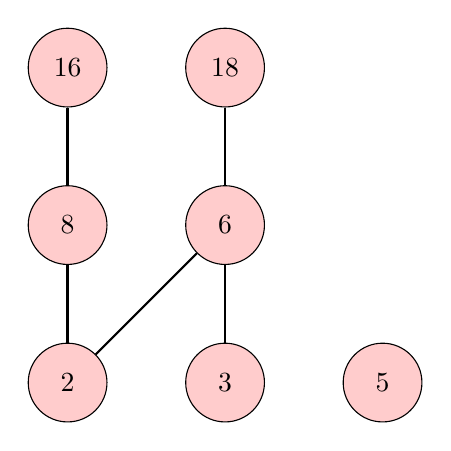
\begin{tikzpicture}[auto,node distance=2cm,main node/.style={circle,fill=red!20,draw,minimum size=1cm}]
  
  \node[main node] (16) {16};
  \node[main node] (18) [right of=16] {18};
  \node[main node] (8) [below of=16] {8};
  \node[main node] (6) [below of=18] {6};
  \node[main node] (2) [below of=8] {2};
  \node[main node] (3) [below of=6] {3};
  \node[main node] (5) [right of=3] {5};
 
  \path[thick]
    (2) edge  node {} (8)
    	edge  node {} (6)
    (3) edge  node {} (6)
    (8) edge  node {} (16)
    (6) edge  node {} (18);	
\end{tikzpicture}
%\end{document}       
\caption{Diagrama de Hasse}
\label{hasse}
\end{figure}

\newpage

En éste caso, no tenemos ni máximo ni mínimo ya que no hay ningun elemento de $A$ que acote superior o inferiormente al resto. Puesto que $A\subset \mathbb{N}$ podemos encontrar cotas superiores e inferiores naturales. El $1$  divide al resto, por lo que es una cota inferior de $A_R$. El $720$ es múltiplo de los tres maximales, por lo que es cota superior de $A_R$.\\

\section{Principio de Inducción}

Sea $P(n)$ una proposición matemática en función de un número entero positivo $n\in \mathbb{Z}^+$. Si $P(n)$ puede ser únicamente verdadera o falsa, entonces podemos emplear el principio de inducción:\\

\emph{Si P(1) es cierta, y si suponiendo que P(k) es verdadera se puede demostrar que P(k+1) también lo es, entonces $P(n)$ es cierta para todo $n\in \mathbb{Z}^+$.}

\subsubsection*{Ejemplo:}
Demostrar que la siguiente ecuación es cierta:

$$
\sum_{i=1}^n i= 1+2+3+\dots+n= \frac{n(n+1)}{2} \quad \forall n \in \mathbb{N}^*
$$

Comprobamos que para $n=1$ es cierto.

$$
\sum_{i=1}^1 i= 1 =\frac{1(1+1)}{2}
$$

Supongamos que para $n=k$ es cierto.

$$
\sum_{i=1}^k i= \frac{k(k+1)}{2}
$$

Para $n=k+1$ tenemos que:

$$
\sum_{i=1}^{k+1} i= \sum_{i=1}^k i + (k+1) = \frac{k(k+1)}{2} + (k+1) =\frac{(k+1)(k+2)}{2}
$$

\section{Aplicaciones}
Dados dos conjuntos $A$ y $B$, una función o aplicación $f:A\rightarrow B$ es un caso particular de relación binaria que asocia a cada  $a\in A$ un único objeto $b\in B$, que se denomina imagen de $a$ y se denota por $b=f(a)$.\\

Al conjunto de los elementos de A para los cuales existe imagen se denomina dominio de la función y se denota por $Dom(f)$.\\

Al conjunto de todas las imágenes de A se denomina imagen de la función y se denota por $Im(f)$.
$$
Im(f)=f(A)=B
$$

Se define la imagen reciproca de de $b\in B$ como el conjunto de los elementos de $A$ cuya imagen es $b$. Se denota por $f^{-1}(b)$.

$$
f^{-1}(b):=\lbrace a \in A : f(a) = b \rbrace
$$

\subsection*{Tipos de aplicaciones}
\begin{itemize}
\item \textbf{Aplicación inyectiva: }Una aplicación es inyectiva si no hay dos objetos del dominio con la misma imagen.
$$
f(x)=f(y)\Longleftrightarrow x=y
$$
\item \textbf{Aplicación sobreyectiva: }Una aplicación es sobreyectiva si todos los objetos de B son imagen de almenos un objeto de A:
$$
\forall b\in B \ \exists \ a\in A / f(a)=b \Longleftrightarrow Im(f)=B
$$
\item \textbf{Aplicación biyectiva:} Una función es biyectiva si es sobreyectiva e inyectiva a la vez. Por tanto, todos los elementos de $A$ tienen una imagen distinta en $B$ y a cada $b\in B$ le corresponde un único elemento $a \in A$.
\end{itemize}

Para las aplicaciones biyectivas existe una aplicación o \textbf{función inversa}, denotada por $f^{-1}$, tal que
$$
f^{-1}(b)=a
$$

\subsection*{Composición de aplicaciones}
Sean $f:A\rightarrow B$ y $g:C \rightarrow D$ dos aplicaciones con $B \subset C$. Se denomina función o aplicación compuesta a
$$
(g\circ f)(a)\equiv g(f(a))
$$

\subsubsection*{Propiedades:}
\begin{itemize}
\item Asociativa:\quad $ h \circ (g \circ f)=(h \circ g) \circ f$
\item No conmutativa en general.
\item La composición de aplicaciones inyectivas es una aplicación inyectiva.
\item La composición de aplicaciones sobreyectivas es una aplicación sobreyectiva.
\item La composición de aplicaciones biyectivas es una aplicación biyectiva.
\end{itemize}

\end{document}
